% !TEX program = pdflatex
% Compile from the project root so that "outputs/..." paths resolve.
\documentclass[11pt]{article}

% ── Layout ────────────────────────────────────────────────────────────────────
\usepackage[margin=1in]{geometry}
\usepackage{microtype}
\usepackage{parskip}
\usepackage{float}           % [H] float specifier
\usepackage{tikz}
\usetikzlibrary{arrows.meta, positioning}

% ── Fonts ─────────────────────────────────────────────────────────────────────
\usepackage[T1]{fontenc}
\usepackage{lmodern}
\usepackage{newtxtext}
\usepackage[scaled=0.92]{inconsolata}

% ── Math / symbols ────────────────────────────────────────────────────────────
\usepackage{amsmath}
\usepackage{amssymb}

% ── Graphics, color, tables ───────────────────────────────────────────────────
\usepackage{graphicx}
\usepackage{xcolor}
\usepackage{booktabs}
\usepackage{array}
\usepackage{caption}
\usepackage{subcaption}

% ── Boxes for callouts ────────────────────────────────────────────────────────
\usepackage[most]{tcolorbox}

% ── Hyperlinks ────────────────────────────────────────────────────────────────
\usepackage{hyperref}

% ── Color palette ─────────────────────────────────────────────────────────────
\definecolor{accent}{HTML}{2E5A88}        % deep blue
\definecolor{accentred}{HTML}{C44E52}     % warm red (diagram highlights)
\definecolor{softgray}{HTML}{F5F5F7}      % callout background
\definecolor{rule}{HTML}{B7C2D0}          % thin separator
\definecolor{codebg}{HTML}{F2F4F7}        % inline code background

% ── Section formatting ────────────────────────────────────────────────────────
\usepackage{titlesec}
\titleformat{\section}
  {\color{accent}\Large\bfseries\sffamily}
  {\thesection}{0.6em}{}
  [\vspace{-2pt}{\color{rule}\titlerule[0.6pt]}]
\titleformat{\subsection}
  {\color{accent}\large\bfseries\sffamily}
  {\thesubsection}{0.5em}{}
\titlespacing*{\section}{0pt}{1.4em}{0.6em}

% ── Caption styling ───────────────────────────────────────────────────────────
\captionsetup{font=small, labelfont={bf,color=accent}, skip=4pt}

% ── Hyperref styling ──────────────────────────────────────────────────────────
\hypersetup{colorlinks=true, linkcolor=accent, urlcolor=accent, citecolor=accent}

% ── Inline code ───────────────────────────────────────────────────────────────
\newcommand{\code}[1]{%
  \tcbox[on line, colback=codebg, colframe=codebg,
         boxrule=0pt, arc=2pt, left=2pt, right=2pt, top=0pt, bottom=0pt]
        {\ttfamily\small #1}}

% ── Callout box ───────────────────────────────────────────────────────────────
\newtcolorbox{keybox}[1][]{
  enhanced, breakable,
  colback=softgray, colframe=accent,
  boxrule=0pt, leftrule=3pt,
  arc=2pt, left=10pt, right=10pt, top=6pt, bottom=6pt,
  fonttitle=\bfseries\sffamily\color{accent},
  #1
}

% ── Title block ───────────────────────────────────────────────────────────────
\title{\vspace{-2.0em}{\color{accent}\textsf{\bfseries K-means Clustering for Authorship Stylometry}}}
\author{}
\date{}

\begin{document}
\maketitle
\vspace{-3.0em}

\noindent
\textit{Given a set of articles written by $K$ authors, how well can we recover
the author groups using only writing style? Perhaps the most natural algorithm
to study this question is K-means.}

% =============================================================================
\section{Clustering 10 Authors}

\paragraph{Dataset and preprocessing.}
We use the \textit{LessWrong 10 Authors} dataset: 10 authors, 40 articles
each, evenly split across two periods (20 from $\leq 2022$, 20 from
$\geq 2024$). To keep article length from masking the stylistic signal, we
truncate every article to its first \textbf{1{,}526 words}, the global minimum
length across the entire cleaned corpus, and discard anything past the cutoff.

\paragraph{Feature extraction.}
We extract \textbf{107} known stylometric features per article using
\code{NLTK} for tokenisation and POS-tagging (with a regex fallback when NLTK
is unavailable). The features fall into seven groups:
\begin{itemize}\setlength\itemsep{1pt}
  \item \textbf{Word and sentence length} statistics (mean, standard deviation,
        median, fractions of 1--6 character words, etc.)
  \item \textbf{Vocabulary richness}: type-token ratio, hapax ratio, Yule~$K$,
        Simpson~$D$, Brunét~$W$, Honoré~$R$
  \item \textbf{Function-word frequencies}: usage rate of each of the top-50
        English function words (``the'', ``and'', ``I'', ``you'', \ldots)
  \item \textbf{Stylistic word categories}: rates for hedges, amplifiers,
        discourse markers, and conjunctions
  \item \textbf{Punctuation rates}: commas, periods, semicolons, parentheses, etc.
  \item \textbf{Coarse POS-tag distributions}: noun, verb, adjective, adverb,
        pronoun, determiner, preposition, conjunction, modal fractions
  \item \textbf{Character-level ratios}: uppercase fraction, vowel frequencies
\end{itemize}
Features with zero variance across the corpus are dropped; the rest are
z-scored with \code{sklearn}'s \code{StandardScaler} so every feature has mean
0 and standard deviation 1 before clustering.

\paragraph{Clustering.}
We run \code{sklearn.cluster.KMeans} with $K=10$,
\code{init="k-means++"}, and \code{n\_init=10}: the algorithm makes ten
independent attempts and returns the one with the lowest \textbf{within-cluster
sum of squares}, the \emph{distortion}
\[
  L \;=\; \sum_{k=1}^{K} \sum_{\mathbf{x} \in C_k}
          \lVert \mathbf{x} - \boldsymbol{\mu}_k \rVert^2,
\]
where $C_k$ is the set of articles assigned to cluster $k$ and
$\boldsymbol{\mu}_k$ is its centroid.

\paragraph{Measuring performance: the Adjusted Rand Index.}
A natural measure of clustering quality compares the cluster
assignments against the true author labels by examining every \emph{pair} of
articles. For a dataset of $n$ articles there are $\binom{n}{2}$ such pairs.
For each pair, the clustering either \textbf{agrees} with the ground truth
(both labellings put the two articles in the same group, or both put them in
different groups) or it \textbf{disagrees}. The \textbf{Rand Index (RI)} is
simply the fraction of pairs on which the clustering agrees:
\[
  \mathrm{RI}
  = \frac{\text{number of agreeing pairs}}{\displaystyle\binom{n}{2}}.
\]
The problem is that even a random clustering achieves a high RI. With ten
authors and 400 articles most pairs are from different authors; a random
partition will still separate them most of the time, racking up agreements
for free. The \textbf{Adjusted Rand Index (ARI)} subtracts the agreement
expected from a random partition, rescaling so that random chance scores
exactly 0:
\begin{itemize}\setlength\itemsep{1pt}
  \item \textbf{ARI $= 1$}: perfect recovery of the true author groups.
  \item \textbf{ARI $\approx 0$}: no better than random chance.
  \item \textbf{ARI $< 0$}: systematically worse than random.
\end{itemize}

It is worth noting that ARI depends only on which pairs of points are grouped together or separated, not on the labels assigned to the clusters.

\paragraph{Results.}
The 400-article input matrix is $400 \times 107$ after feature extraction.

\begin{figure}[H]
  \centering
  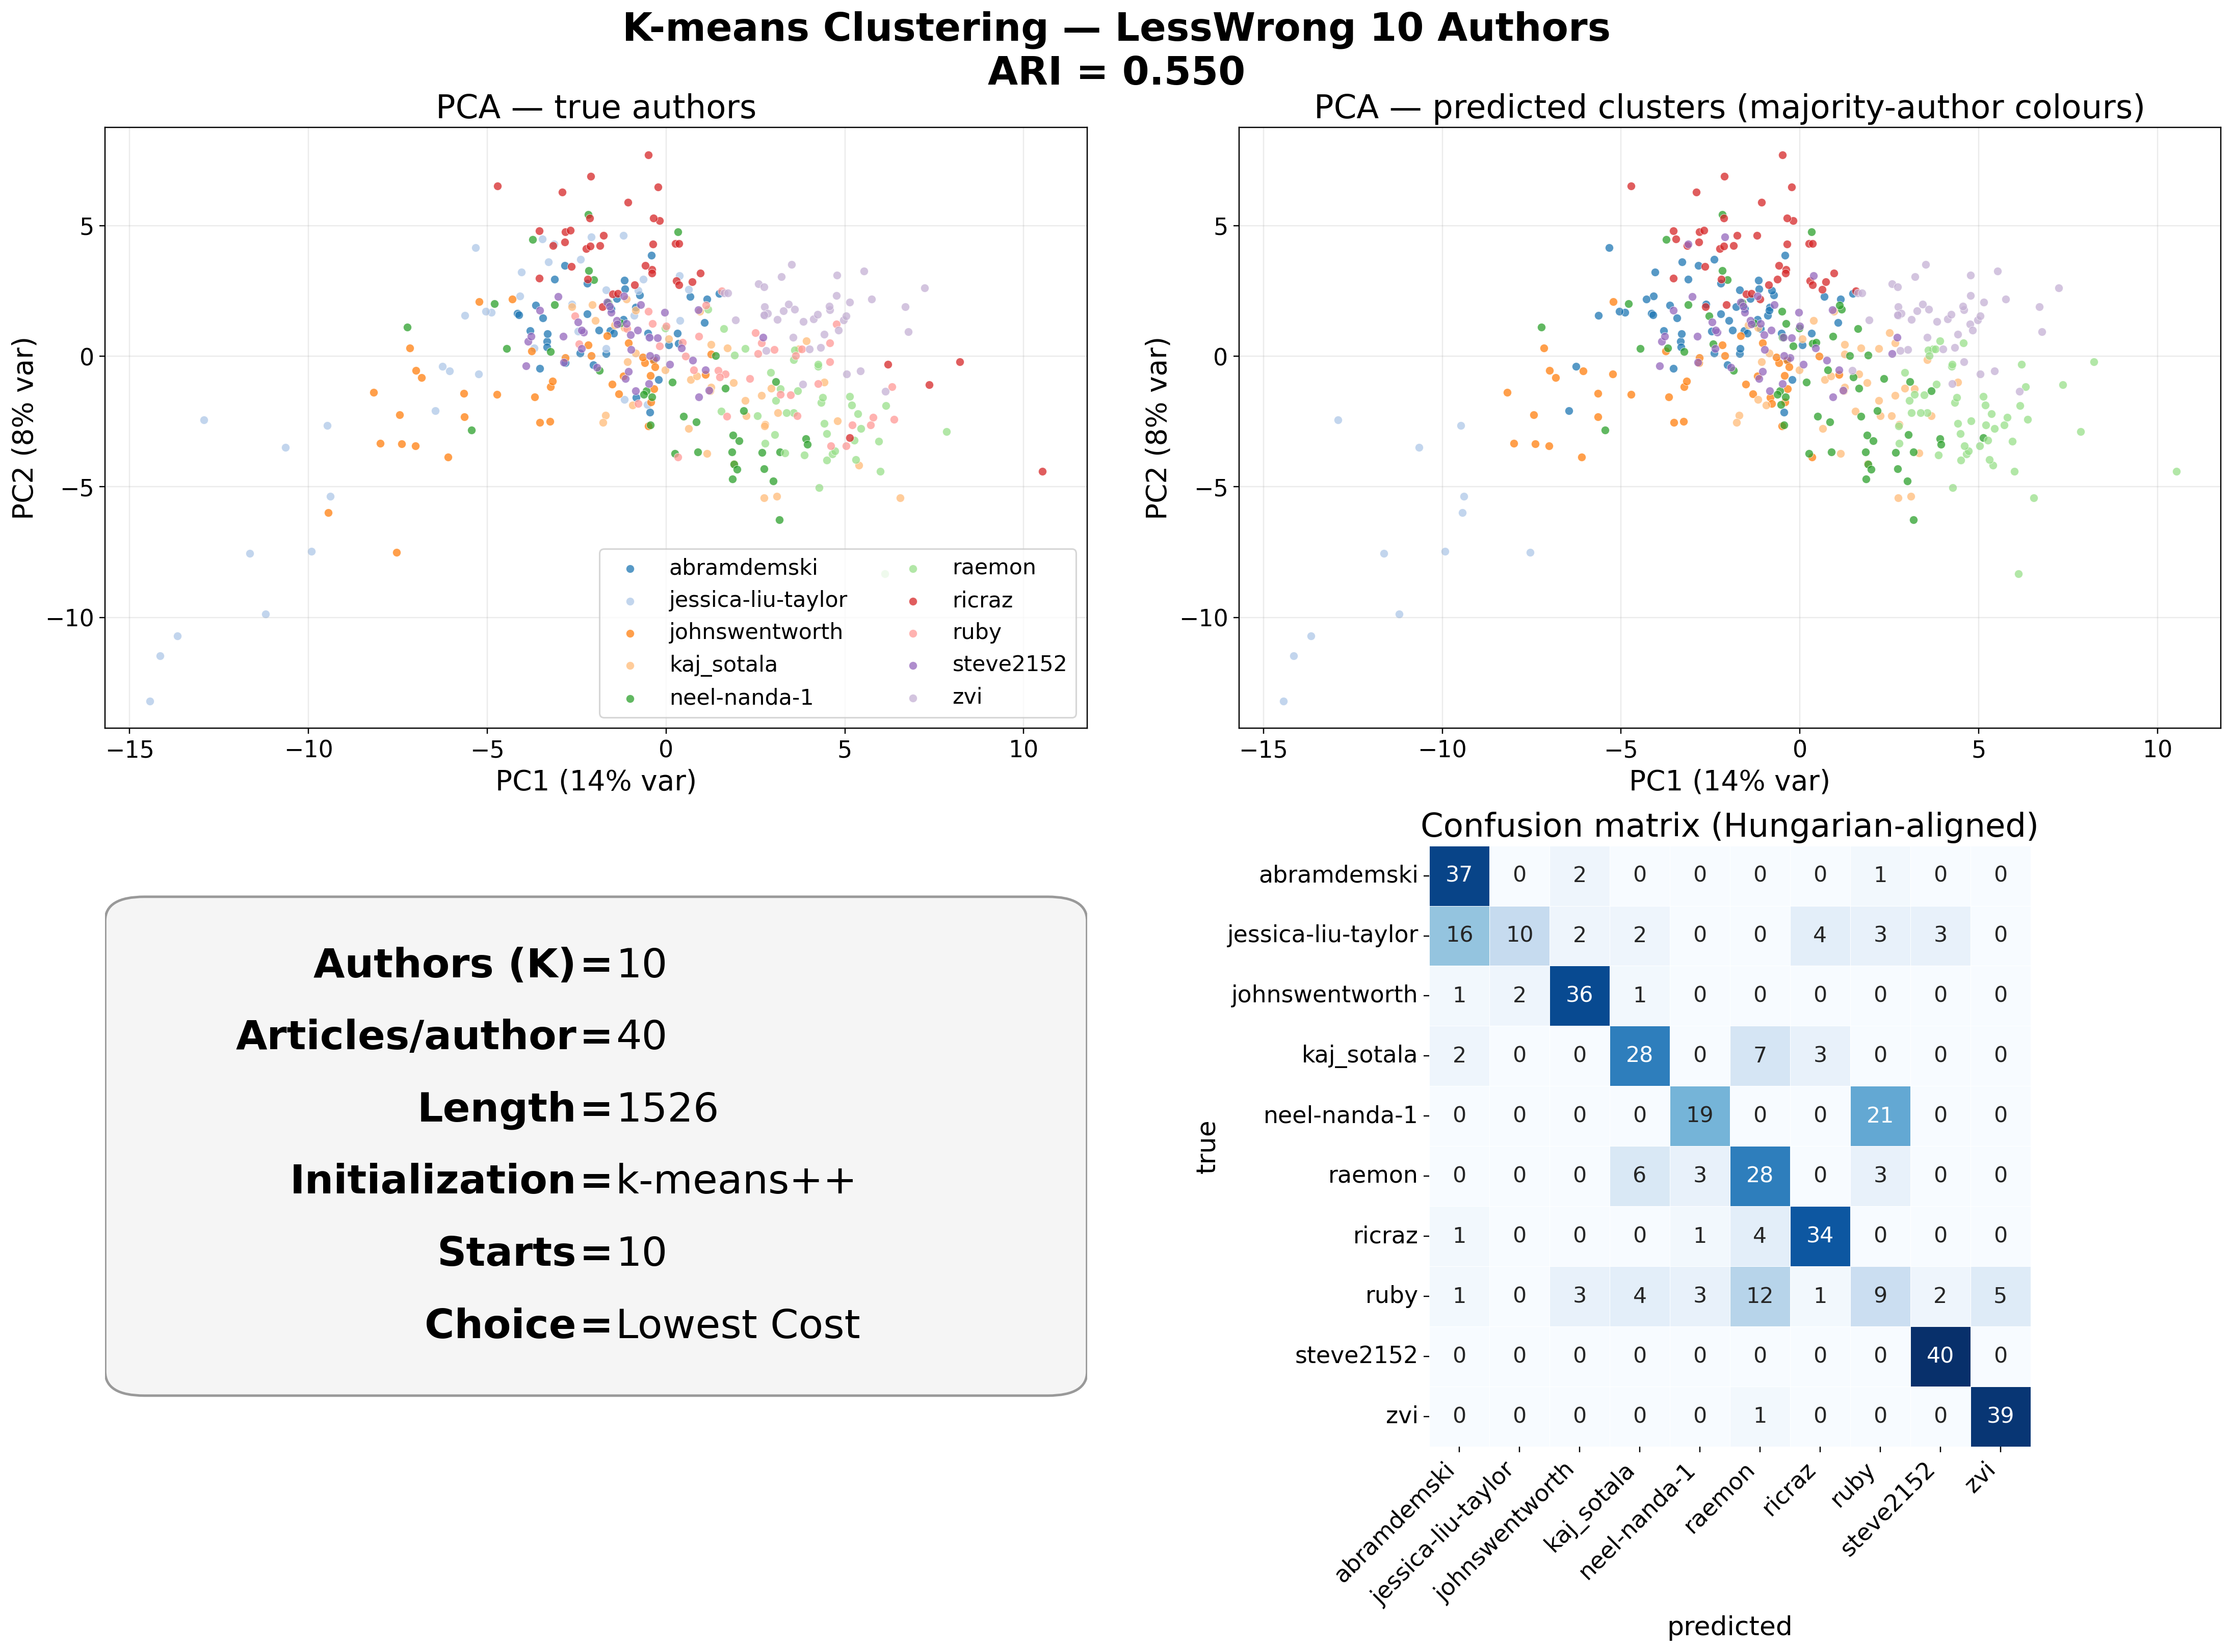
\includegraphics[width=0.82\linewidth]{../outputs/kmeans/cluster_10/clustering.png}
  \caption{K-means on the LessWrong 10 Authors dataset, $K=10$. \textit{Top
  left}: articles projected onto the two PCA directions of largest variance
  (\code{sklearn.decomposition.PCA} applied to the centered, z-scored matrix),
  coloured by true author. \textit{Top right}: same projection, coloured by
  predicted cluster (each cluster takes the colour of its majority author).
  \textit{Bottom right}: confusion matrix after a Hungarian one-to-one
  alignment (\code{scipy.optimize.linear\_sum\_assignment}) between predicted
  clusters and true authors.}
  \label{fig:cluster10}
\end{figure}

The clustering achieves \textbf{ARI = 0.55}, which is fairly impressive given
that we are trying to separate ten groups simultaneously. The confusion matrix
shows a prominent diagonal: most authors land mostly in their own cluster.

Despite this strong result, a question remains: if we were to run the exact
same experiment again, would we still see a similar ARI? K-means is a
randomized algorithm. To cluster the articles, it must first place $K$ initial
centroids somewhere in the feature space. Different starting positions lead to
different final clusters, and the algorithm can get stuck in different local
minima of $L$. \textbf{k-means++} is a smarter initialization strategy than
placing centroids uniformly at random: it places each subsequent centroid with
probability proportional to its squared distance from the nearest centroid
already chosen, biasing the starting configuration toward spread-out positions
and improving convergence. But k-means++ is still random.

The randomness is controlled by a single integer called the \emph{master seed}
(\code{random\_state} in sklearn). Given a seed, sklearn generates a fully
deterministic sequence of random numbers. For each of the \code{n\_init=10}
attempts, k-means++ draws the next values from this sequence to select $K$
starting centroids. The ten attempts therefore use different starting centroids
(drawn sequentially from the same seed's stream), each converges independently
to some local minimum, and each records its own distortion $L_i$. sklearn
returns the attempt $i^* = \arg\min_i L_i$ with the lowest distortion, for which ARI is calculated.

The key issue is that all ten attempts are tied to one seed. Change the seed,
and sklearn generates a different random-number sequence, produces a different
pool of ten starting configurations, and may return a different ``best''
clustering with a different ARI. With \code{random\_state=42} we obtained
ARI $= 0.55$, but without running other seeds we cannot tell whether this is
a typical outcome or a lucky one. To measure the variability, we treat each
seed as an independent trial: for ten seed values $(42, 100, 200, \ldots, 900)$
we run the same experiment and record the ARI of the lowest-distortion attempt.
Figure~\ref{fig:seed_diagram} illustrates the procedure.

\begin{figure}[H]
\centering
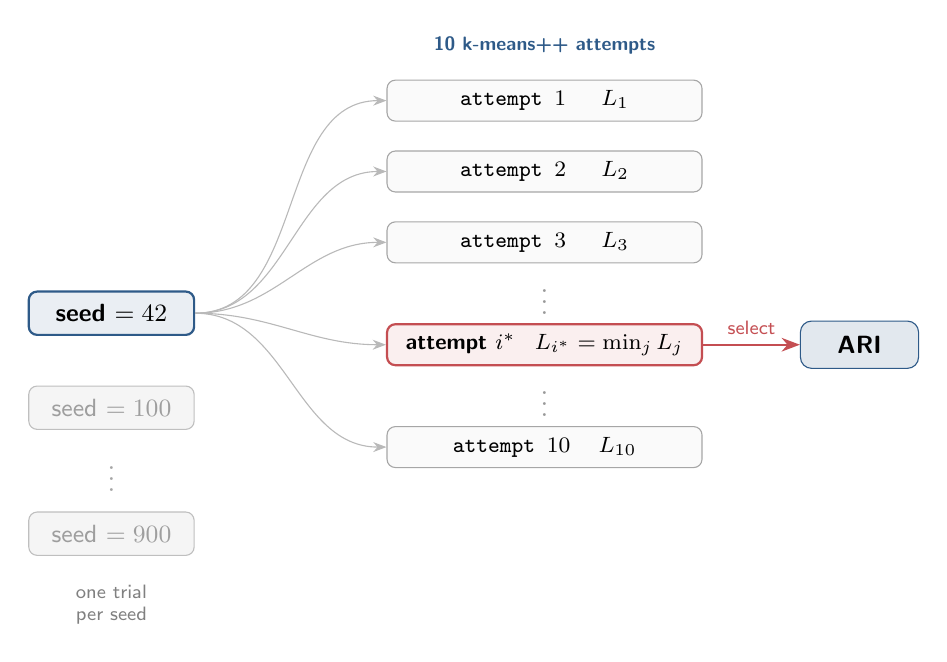
\begin{tikzpicture}[
  seedbox/.style={
    draw=accent, fill=accent!10, rounded corners=3pt,
    minimum width=2.1cm, minimum height=0.55cm,
    align=center, font=\small\sffamily\bfseries, thick
  },
  fadedseed/.style={
    draw=black!25, fill=black!4, rounded corners=3pt,
    minimum width=2.1cm, minimum height=0.55cm,
    align=center, font=\small\sffamily, text=black!38
  },
  trybox/.style={
    draw=black!35, fill=gray!4, rounded corners=3pt,
    minimum width=4.0cm, minimum height=0.52cm,
    align=center, font=\footnotesize\ttfamily
  },
  bestbox/.style={
    draw=accentred, fill=accentred!9, rounded corners=3pt,
    minimum width=4.0cm, minimum height=0.52cm,
    align=center, font=\footnotesize\sffamily\bfseries, thick
  },
  aribox/.style={
    draw=accent, fill=accent!14, rounded corners=4pt,
    minimum width=1.5cm, minimum height=0.6cm,
    align=center, font=\small\sffamily\bfseries
  },
  garr/.style={->, >=Stealth, gray!55, thin},
  barr/.style={->, >=Stealth, accentred, thick},
]

%% ── Left column: seeds ──────────────────────────────────────────────────────
\node[seedbox]   (s42)  at (0,  2.8) {seed $= 42$};
\node[fadedseed] (s100) at (0,  1.6) {seed $= 100$};
\node[text=black!35, font=\normalsize] at (0, 0.8) {$\vdots$};
\node[fadedseed] (s900) at (0,  0.0) {seed $= 900$};
\node[font=\scriptsize\sffamily, text=black!50, align=center]
  at (0, -0.9) {one trial\\per seed};

%% ── Middle column: 10 attempts from seed 42 ─────────────────────────────────
\node[font=\scriptsize\sffamily\bfseries, text=accent, align=center]
  at (5.5, 6.2) {10 k-means++ attempts};

\node[trybox]  (a1)    at (5.5, 5.5) {attempt $1$\hspace{1.5em}$L_1$};
\node[trybox]  (a2)    at (5.5, 4.6) {attempt $2$\hspace{1.5em}$L_2$};
\node[trybox]  (a3)    at (5.5, 3.7) {attempt $3$\hspace{1.5em}$L_3$};
\node[text=black!40, font=\normalsize] at (5.5, 3.05) {$\vdots$};
\node[bestbox] (abest) at (5.5, 2.4)
  {attempt $i^*$\hspace{0.8em}$L_{i^*} = \min\nolimits_j L_j$};
\node[text=black!40, font=\normalsize] at (5.5, 1.75) {$\vdots$};
\node[trybox]  (a10)   at (5.5, 1.1) {attempt $10$\hspace{1.2em}$L_{10}$};

%% Arrows: seed 42 → each attempt (fan)
\foreach \a in {a1,a2,a3,abest,a10} {
  \draw[garr] (s42.east) to[out=0, in=180] (\a.west);
}

%% ── Right: ARI output ────────────────────────────────────────────────────────
\node[aribox] (ari) at (9.5, 2.4) {ARI};
\draw[barr] (abest.east) -- node[above, font=\scriptsize\sffamily]{select} (ari.west);

\end{tikzpicture}
\caption{Procedure for one stability trial. The master seed generates a
deterministic random-number sequence; k-means++ draws from it to produce ten
independent starting configurations. Each attempt converges to a local minimum
of $L$, and the one with the lowest distortion $L_{i^*}$ is selected and scored
with ARI. Running ten different seeds gives ten independent ARI measurements.}
\label{fig:seed_diagram}
\end{figure}

\begin{figure}[H]
  \centering
  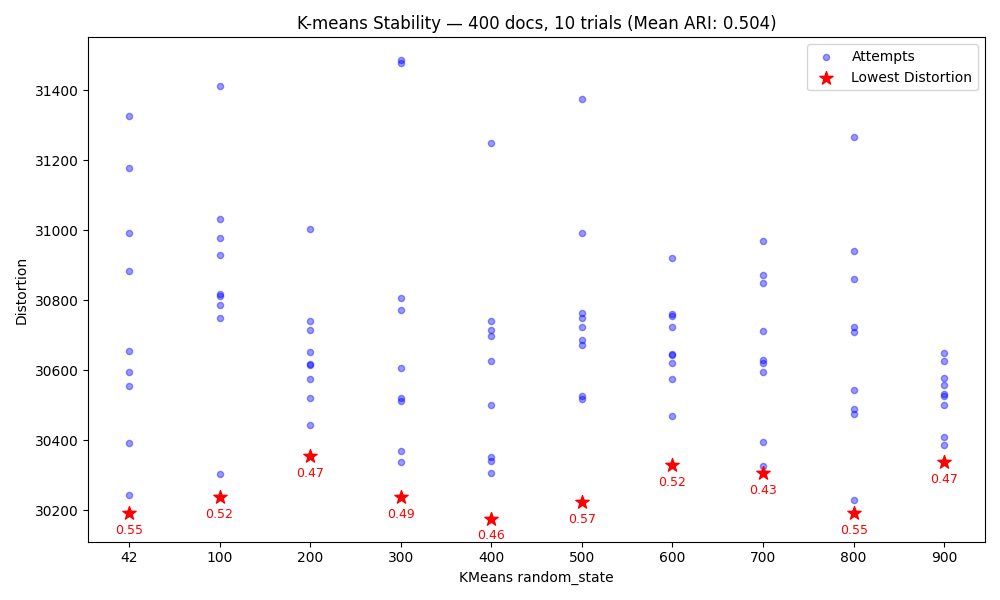
\includegraphics[width=0.78\linewidth]{../outputs/kmeans/cluster_10/ari_vs_seed.png}
  \caption{ARI of the selected attempt (lowest $L$) across ten master seeds.
  Blue dots show the distortions of all ten attempts within each trial; the
  red star marks the one sklearn returns. The annotated value is that run's ARI.}
  \label{fig:seed_stability}
\end{figure}

Across the ten trials the mean ARI is \textbf{0.504}, ranging from \textbf{0.43}
to \textbf{0.57}. Our initial result of 0.55 sits on the luckier side of the
distribution, but it is close to the mean.

\paragraph{Which features are doing the work?}
For every feature we compute the ANOVA F-ratio (between-cluster variance
divided by within-cluster variance) on the predicted clusters using our
\code{f\_ratio} function in \code{src/clustering.py}. A high F-ratio means
the feature separates clusters more than it varies inside them.

\begin{figure}[H]
  \centering
  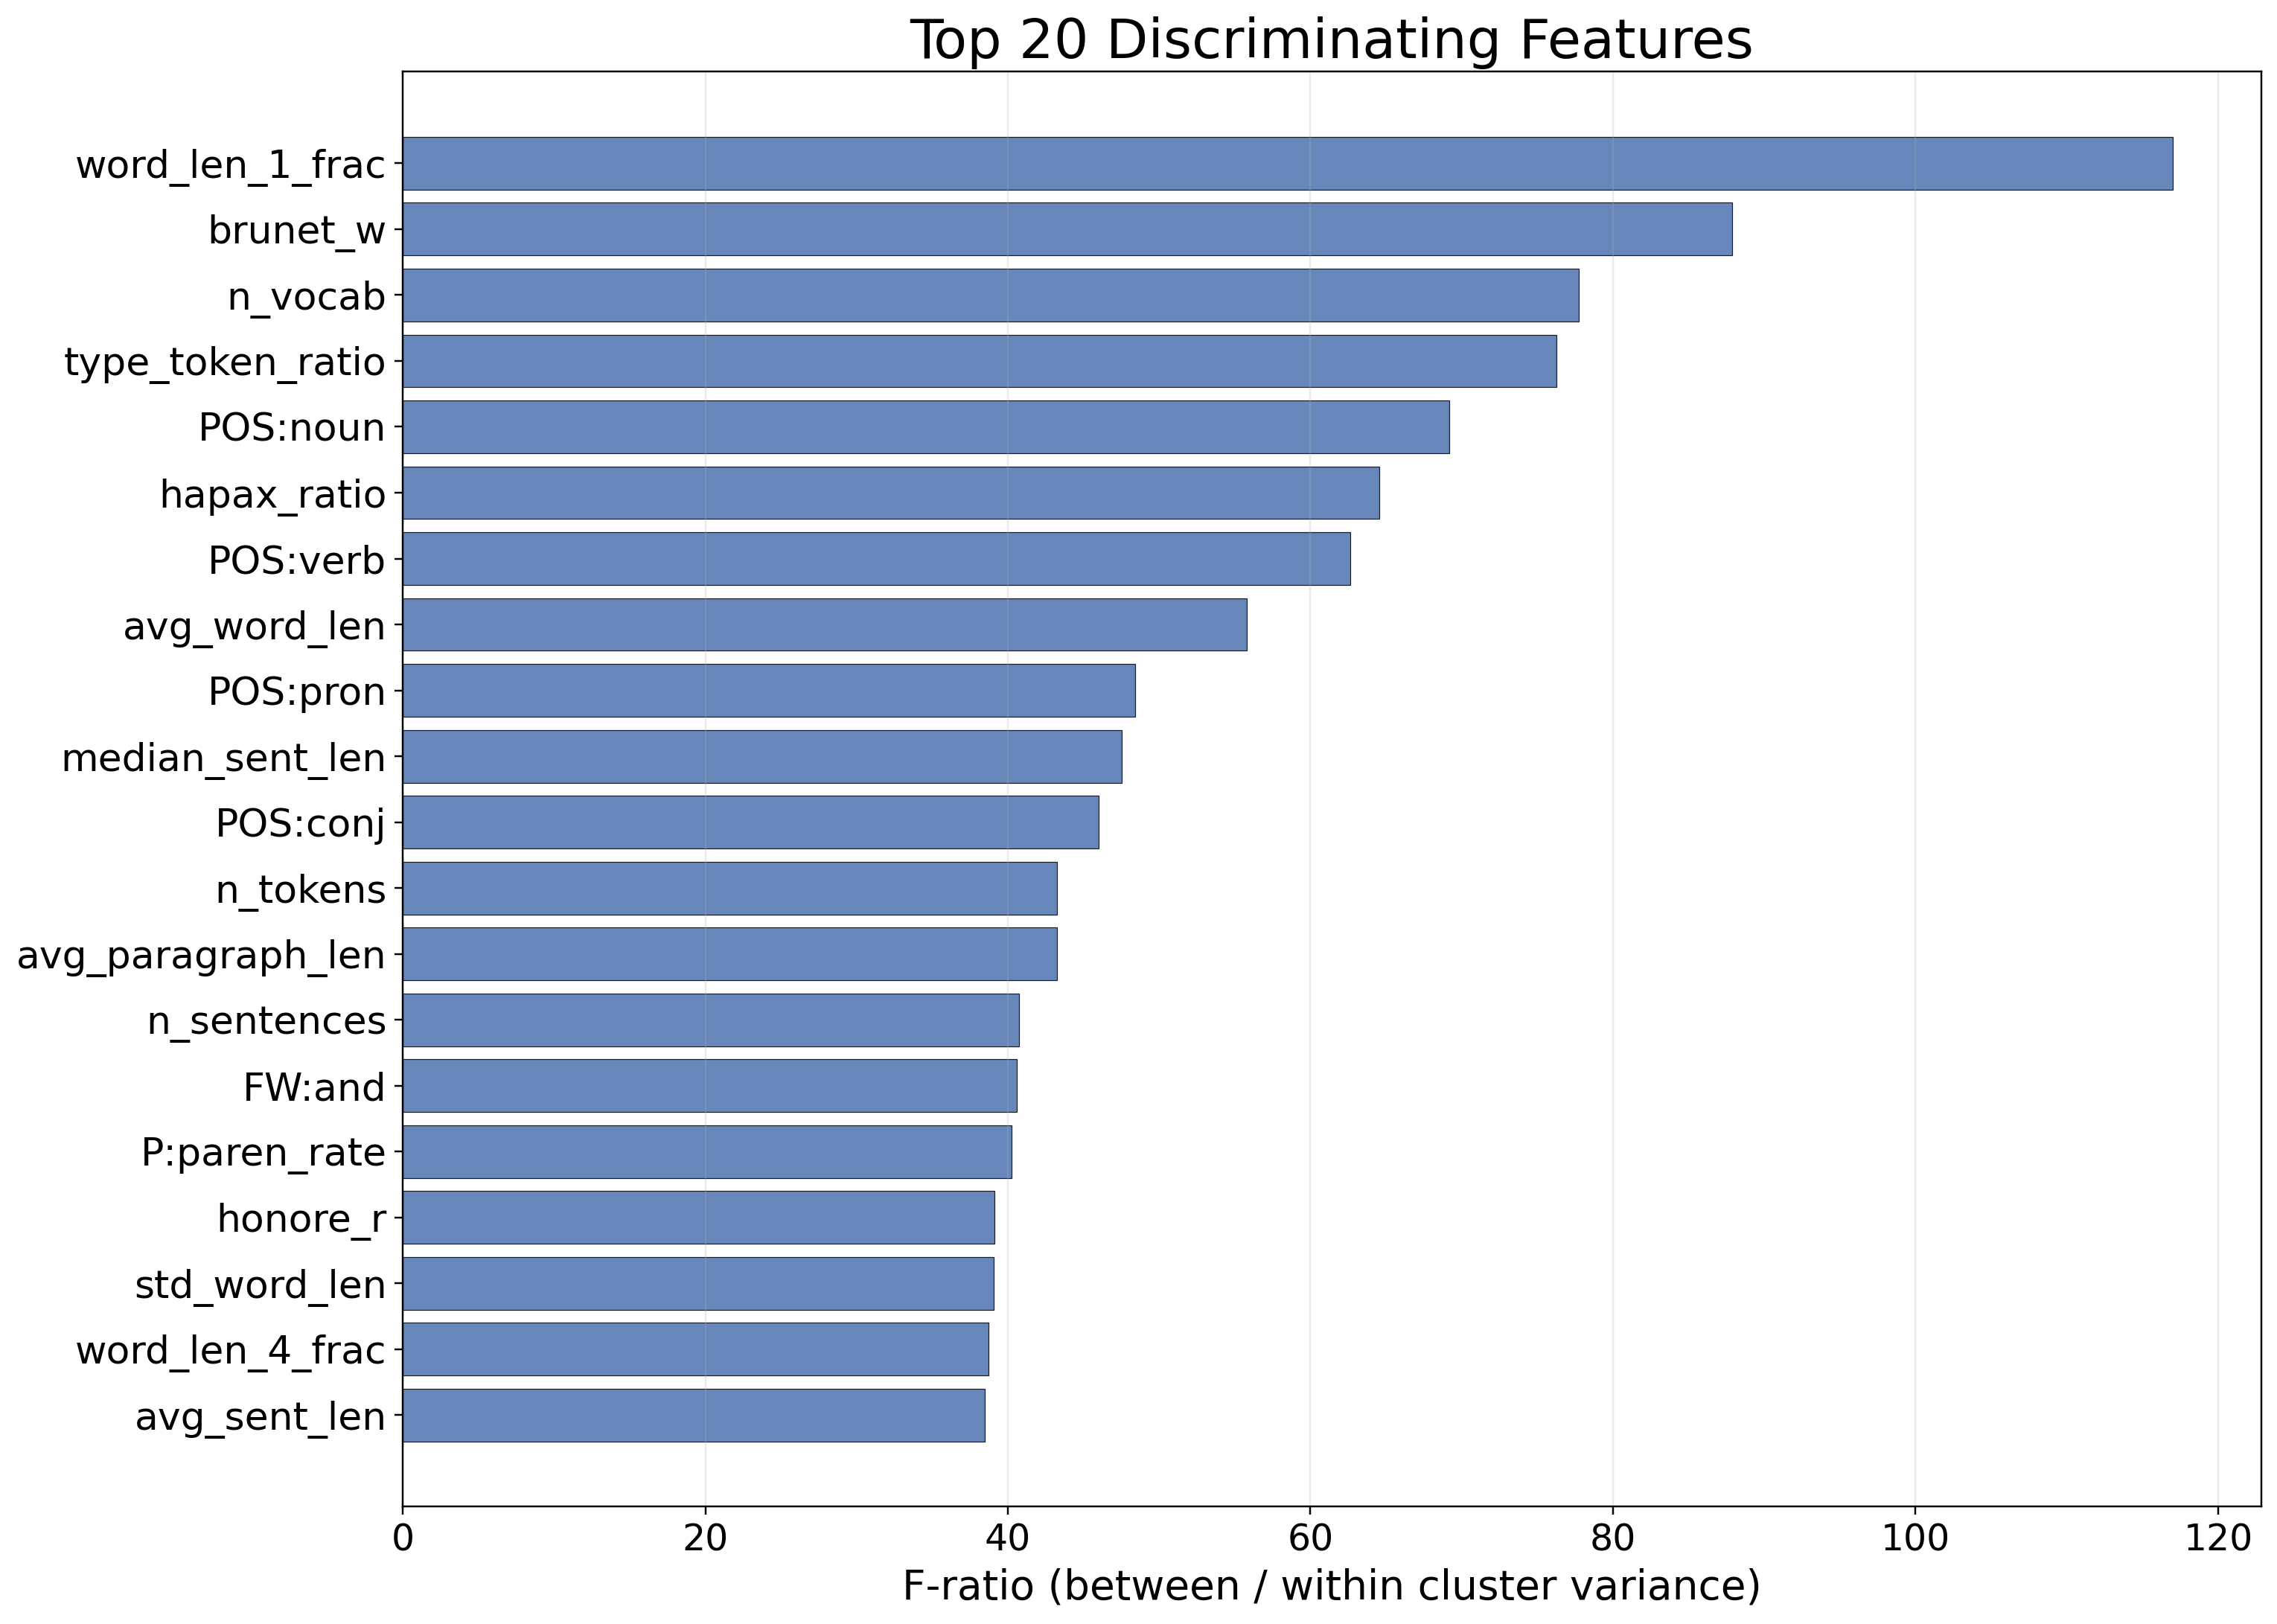
\includegraphics[width=0.72\linewidth]{../outputs/kmeans/cluster_10/top_features.png}
  \caption{Top 20 discriminating features for the $K=10$ clustering, ranked
  by ANOVA F-ratio. Single-character word rate (\code{word\_len\_1\_frac}),
  Brunét's $W$, vocabulary size (\code{n\_vocab}), and POS distributions
  dominate.}
  \label{fig:topfeats}
\end{figure}

The strongest signals are how often an author uses one-letter words (mostly ``I'' and
``a''), vocabulary richness, the noun/verb/pronoun mix, and average word
length. None of these depend on what the article is \textit{about}.

% =============================================================================
\section{Effect of Articles per Author ($M$)}

How does data density, represented by the number of articles per author $M$,
affect performance? An author's writing style varies between articles, often
substantially: they may write across multiple topics and genres, each
dragging the surface features in different directions. An opinion piece tends
to use the word ``I'' more often than a report, for example, and the rate of
``I'' is one of our features. LessWrong articles also carry residual noise
from code blocks, MathJax formulas, image captions, quoted material, and
audio transcripts that are difficult to remove perfectly. With too few
articles per author, the sample likely becomes a poor estimate of that author's true
style, so we expect K-means performance to degrade as $M$ shrinks.

\paragraph{Setup.}
We reuse the \textit{LessWrong 10 Authors} corpus, fix $K=4$ and length $N=1{,}526$
words, and sweep $M \in \{5, 10, 15, 20\}$. For each $M$ we run 50
trials: sample 4 of the 10 authors at random, sample $M$ articles per author,
truncate each at the first N words, extract features, cluster with 10 k-means ++ initializations, select the attempt with the lowest distortion, and record ARI.

\begin{figure}[H]
  \centering
  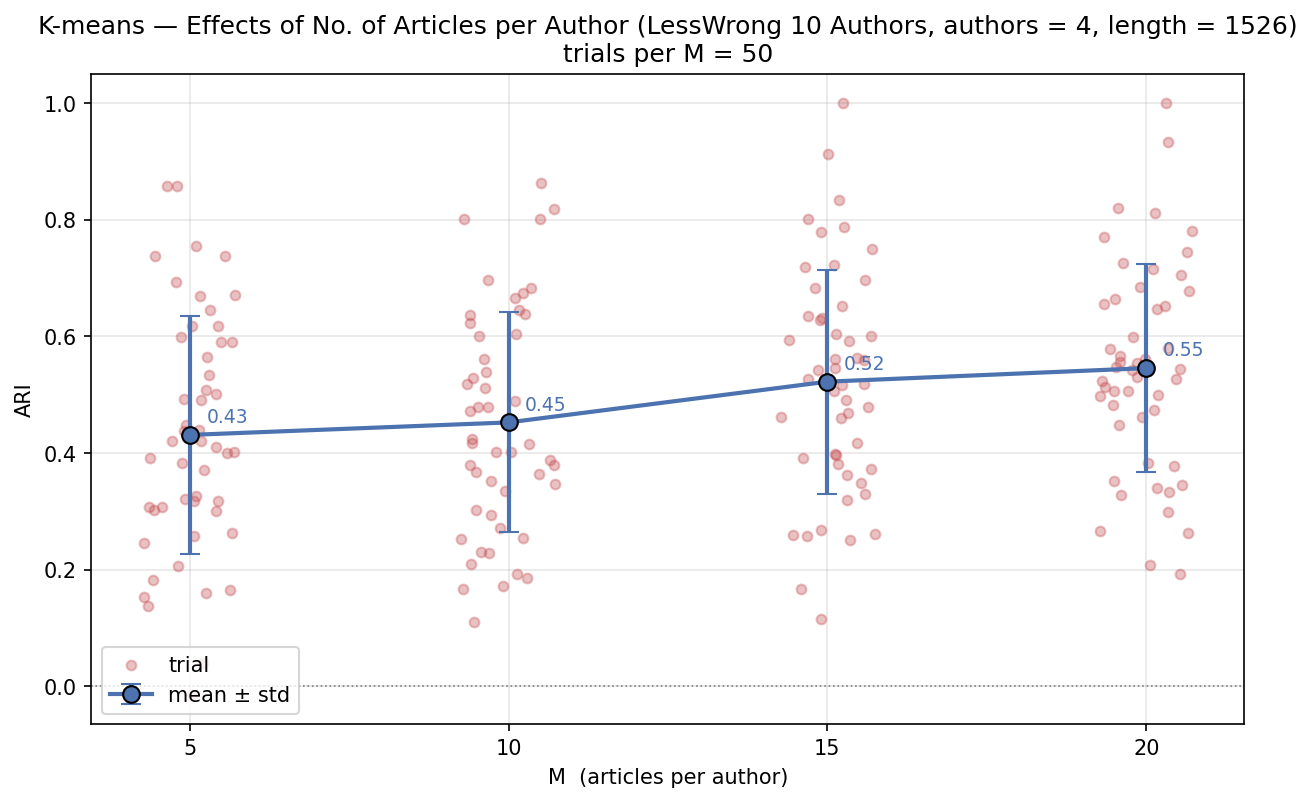
\includegraphics[width=0.82\linewidth]{../outputs/kmeans/effect_of_m/ari_vs_m_10authors.png}
  \caption{ARI vs.\ $M$ on LessWrong 10 Authors ($K=4$, $N=1526$, 50 trials per
  $M$). Mean ARI rises from $0.43$ at $M=5$ to $0.55$ at $M=20$.}
  \label{fig:m10}
\end{figure}

ARI rises steadily from $0.43$ at $M=5$ to $0.55$ at $M=20$, with the curve
still climbing at the upper end of the sweep. It is unclear whether
performance would continue to improve past $M=20$ or eventually saturate.

To study higher values of $M$, the number of articles available per author
needs to be considerably larger than the maximum $M$ we intend to sample.
Otherwise, for large $M$, the articles sampled for each author will largely
overlap across trials, so ARI variability will mostly reflect which author
group was sampled rather than which articles. With 4 authors drawn from 10,
trials already tend to share authors, so that
source of variability is limited to begin with. Finding 10 or more LessWrong authors with
that many qualifying articles (length $\geq 1{,}526$ words) turns out to be
difficult. We therefore restrict to a separate \textit{LessWrong 4 Authors}
dataset, four specific authors for whom we were able to find 76--79 articles
each. While any conclusions will be specific to these four authors, the
results can still hint at whether collecting more articles per author is worth
the effort.

\begin{figure}[H]
  \centering
  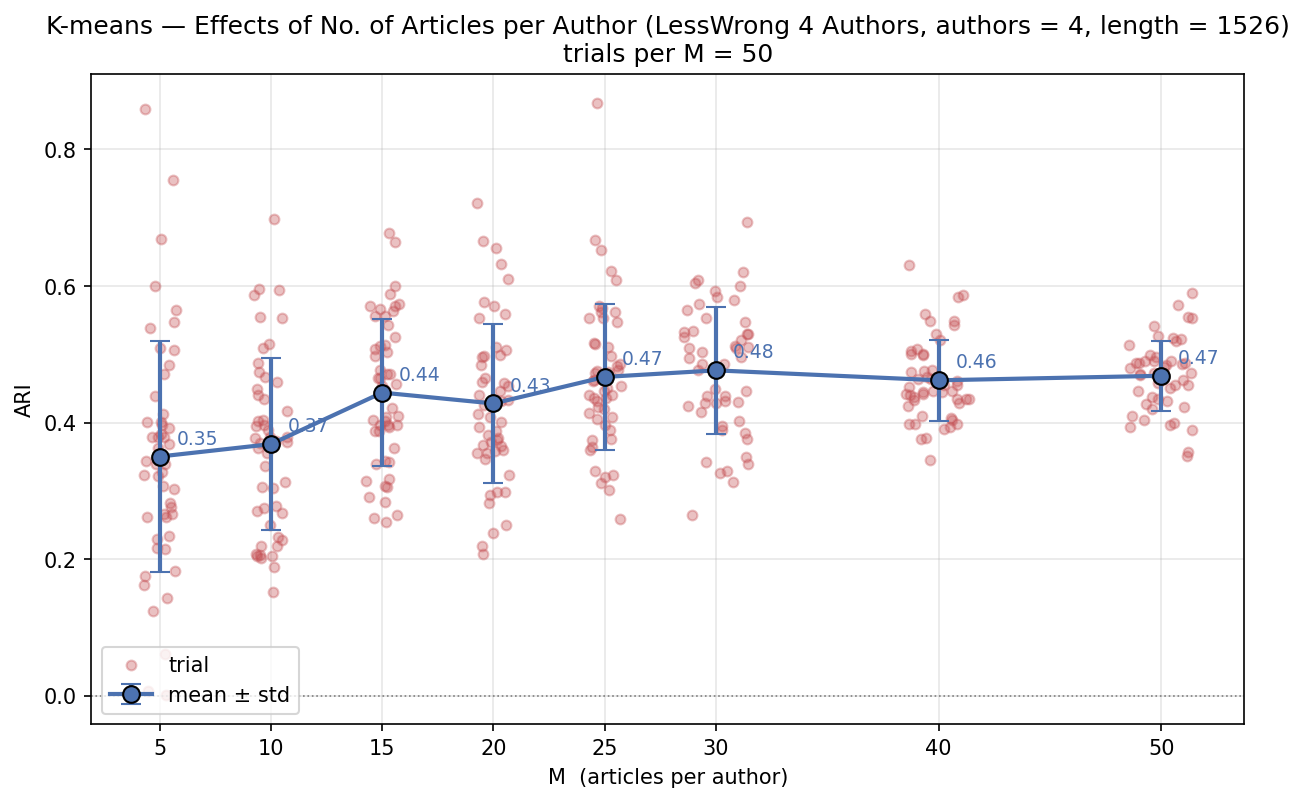
\includegraphics[width=0.82\linewidth]{../outputs/kmeans/effect_of_m/ari_vs_m_4authors.png}
  \caption{ARI vs.\ $M$ on LessWrong 4 Authors ($K=4$, $N=1526$, 50 trials per
  $M$). The curve climbs from $0.35$ at $M=5$ to $\sim 0.48$ near $M=30$, then
  plateaus through $M=40$.}
  \label{fig:m4}
\end{figure}

The pattern closely mirrors the 10-author case: mean ARI climbs from $0.35$
to $\sim 0.48$ as $M$ goes from 5 to 30, then \textbf{flattens} between
$M=30$ and $M=40$, hovering at $0.46$--$0.48$. On this kind of LessWrong corpus, collecting more than roughly
30 articles per author appears to yield little extra clustering quality.

% =============================================================================
\section{Effect of Number of Authors ($K$)}

Does clustering more authors hurt performance? Intuitively yes: the more
authors in the pool, the more likely some pairs of writing styles overlap,
making K-means' task harder. To isolate the effect of $K$ from confounders,
we must hold everything else fixed.

\paragraph{Setup.}
We reuse \textit{LessWrong 10 Authors} and fix $M=15$ articles per author and
$N=1{,}526$ words. For each $K \in \{2, 4, 6, 8, 10\}$ we run 50 trials:
sample $K$ of the 10 authors at random, sample $M=15$ of each chosen
author's 40 articles, truncate, extract features, cluster, record ARI.

\begin{figure}[H]
  \centering
  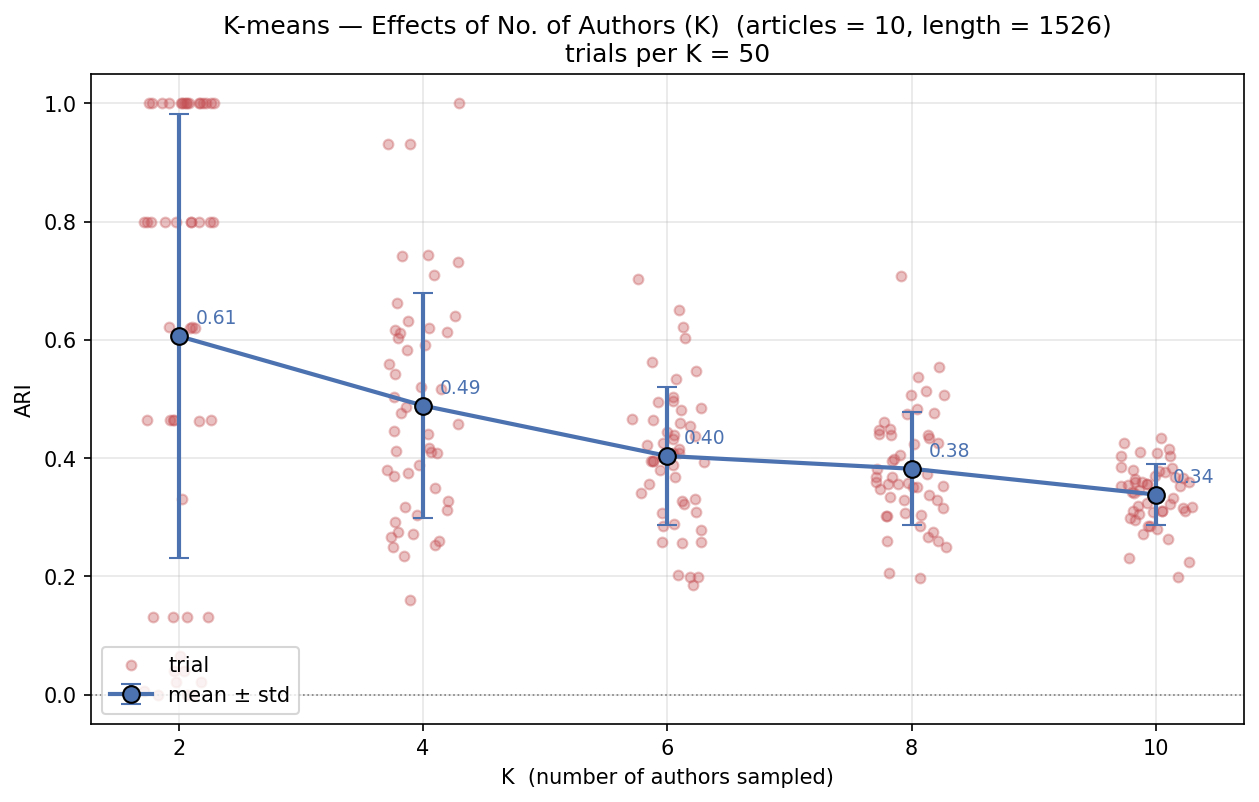
\includegraphics[width=0.82\linewidth]{../outputs/kmeans/effect_of_k/ari_vs_k.png}
  \caption{ARI vs.\ $K$ on LessWrong 10 Authors ($M=15$, $N=1526$, 50 trials
  per $K$). Mean ARI drops monotonically from $0.60$ at $K=2$ to $0.40$ at
  $K=10$.}
  \label{fig:k}
\end{figure}

Within this corpus, the downward trend is clear and monotone, dropping from
$0.60$ at $K=2$ to $0.40$ at $K=10$.

% =============================================================================
\section{Effect of Article Length ($N$)}

How does article length $N$ affect performance? Most of our 107 features are
proportions, frequencies, means: quantities that should be
agnostic to length in expectation, yet noisier when estimated from short
passages.

\paragraph{Setup.}
We use \textit{LessWrong 10 Authors} with $K=5$ and $M=15$, sweeping
$N \in \{100, 200, 500, 1000, 1500\}$. For each $N$ we run 50 trials: sample
5 of the 10 authors, sample 15 articles per author, truncate to the first $N$
words, extract features, run K-means.

\begin{figure}[H]
  \centering
  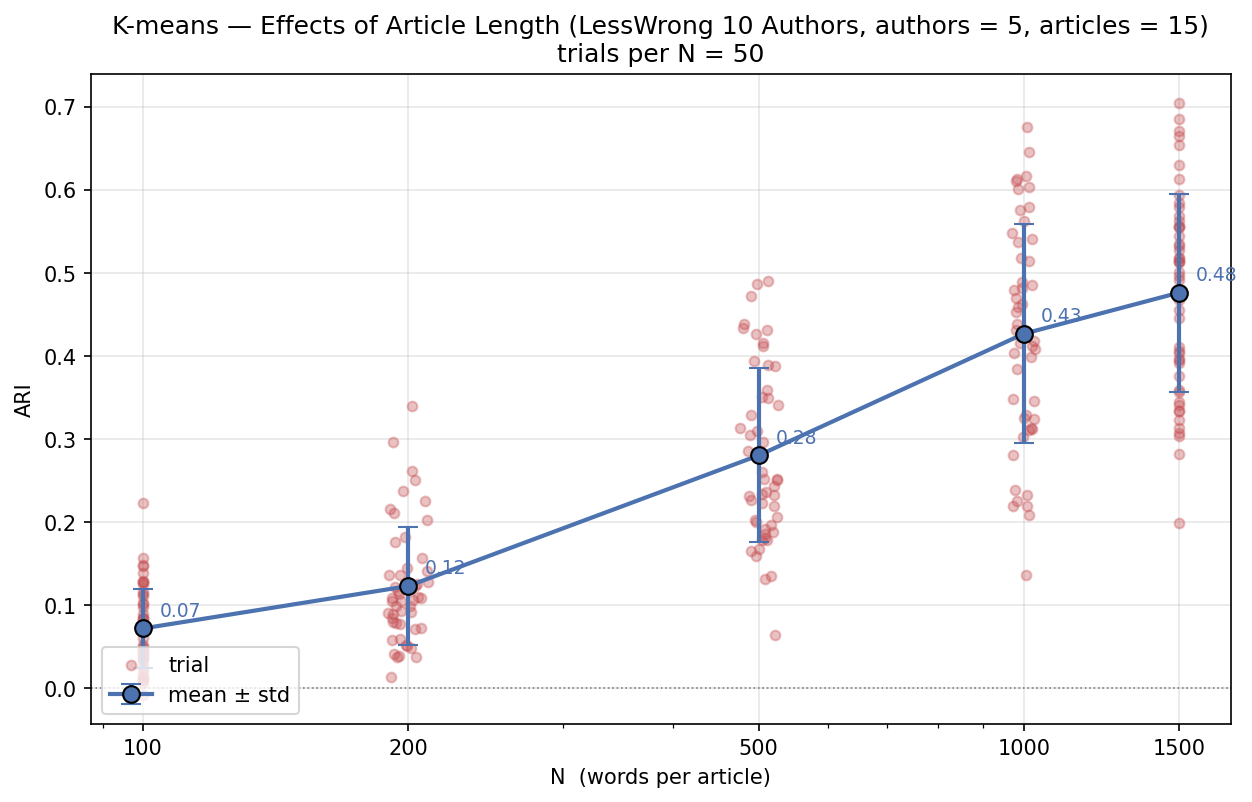
\includegraphics[width=0.82\linewidth]{../outputs/kmeans/effect_of_n/ari_vs_n_10authors.png}
  \caption{ARI vs.\ $N$ on LessWrong 10 Authors ($K=5$, $M=15$, 50 trials per
  $N$). ARI rises steeply from $0.07$ at $N=100$ to $0.48$ at $N=1500$.}
  \label{fig:n10}
\end{figure}

The trend is steep: ARI climbs from $0.07$ at $N=100$ to $0.48$ at
$N=1500$, with the slope easing slightly between $N=1000$ and $N=1500$,
hinting at a plateau that has not yet arrived. To see whether the curve
really flattens, we need longer articles. Finding many long ($\geq
3000$-word) articles for ten LessWrong authors is impractical, so we switch
to a \textit{LessWrong 5 Authors} dataset: five authors for whom we found
35--57 articles each of length $\geq 3{,}000$ words. The setup is identical
except there is no author sampling (all 5 are used each trial) and $N$ now
ranges up to 3{,}000.

\begin{figure}[H]
  \centering
  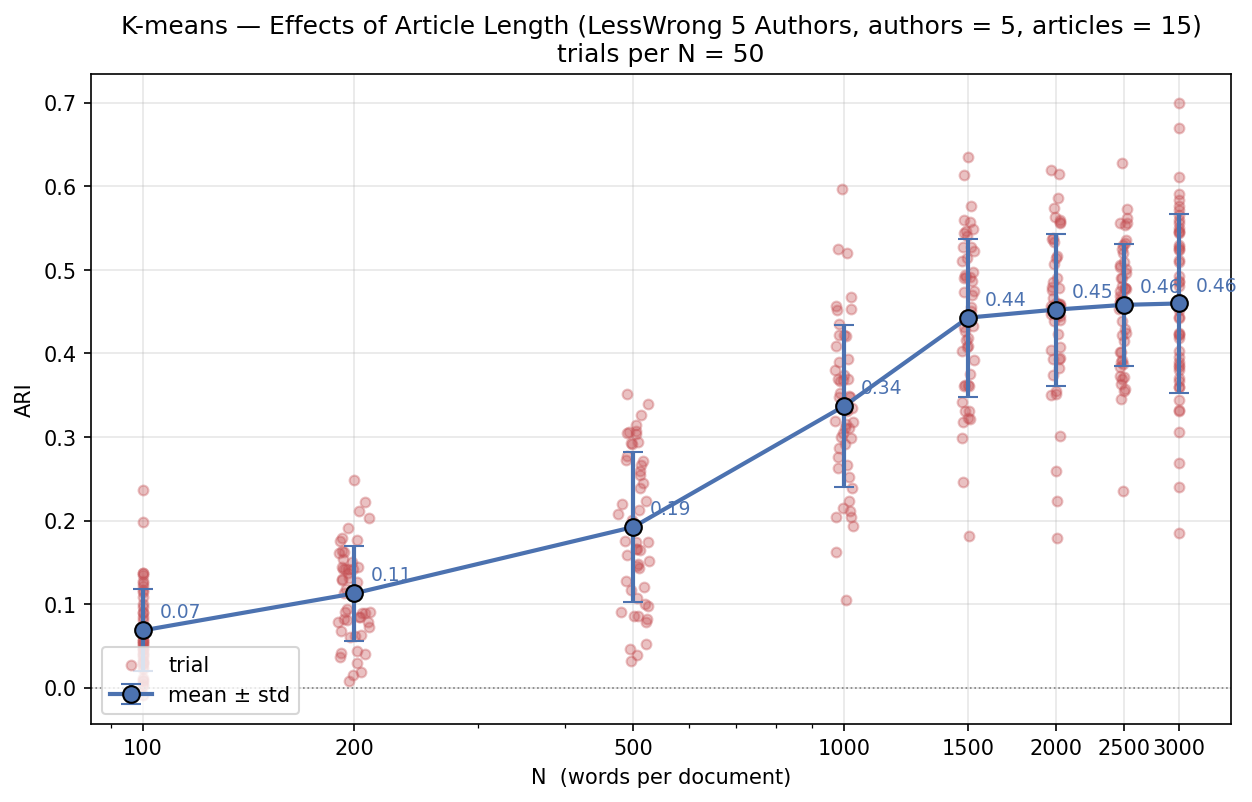
\includegraphics[width=0.82\linewidth]{../outputs/kmeans/effect_of_n/ari_vs_n_5authors.png}
  \caption{ARI vs.\ $N$ on LessWrong 5 Authors ($K=5$, $M=15$, 50 trials per
  $N$). The curve follows the 10-author trend up to $N=1500$, then
  \textbf{flattens}: ARI moves only from $0.44$ to $0.46$ over the range
  $N \in \{1500, 2000, 2500, 3000\}$.}
  \label{fig:n5}
\end{figure}

The shape is striking. Up to $N=1500$ the curve mirrors the 10-author result;
past $N=1500$ it hits a clear break point, barely moving from $0.44$ to
$0.46$ over the next 1{,}500 words. A few possible explanations:

\begin{itemize}\setlength\itemsep{2pt}
  \item \textbf{Feature convergence.} By $N=1500$ most rate-based features may
        already be close to their author means, so the algorithm is hitting a
        performance ceiling for this dataset and feature set.
  \item \textbf{Topic shifts within long articles.} Long articles often span
        multiple sub-discussions; transitions between them can shift the
        stylistic surface. Since we truncate articles from the beginning to the first N words, the break point may reflect an implicit average
        coherent-stretch length of roughly 1{,}500 words.
  \item \textbf{Noisy tails.} Authors often write discursively at the start
        and then move into code blocks, image captions, math, and quoted
        material, all of which add noise to the features.
  \item \textbf{Dataset-specific.} The break point may simply be a property
        of this particular five-author group rather than a general pattern.
\end{itemize}

Regardless, the practical implication is the same: there is little to gain
from chasing articles longer than $\sim 1{,}500$ words for this kind of
clustering problem.

\paragraph{Why does the curve rise in the first place?}
Of our 107 features, roughly 100 are proportions, rates, means, or medians. For each author, these features can be viewed as draws from an underlying author-specific stylistic distribution that is largely independent of article length.
By the Law of Large Numbers, the observed feature values converge toward the author’s true means as sample size increases. At small $N$
each feature is a noisy estimate of the underlying rate, causing articles from
different authors to overlap in feature space.

To make this concrete, we isolate author \code{zvi} from \textit{LessWrong 5 Authors}
and track two features as a function of passage length:

\begin{enumerate}\setlength\itemsep{1pt}
  \item Concatenate all of \code{zvi}'s articles into a single ``master''
        document.
  \item For each window size $N \in \{100, 200, 500, 1000, 1500, 2000, 2500,
        3000\}$, draw 20 random contiguous slices of exactly $N$ tokens.
  \item Compute \code{fw\_you} (rate of the word ``you'') and
        \code{word\_len\_1\_frac} (rate of one-character words) on each
        slice.
\end{enumerate}

\begin{figure}[H]
  \centering
  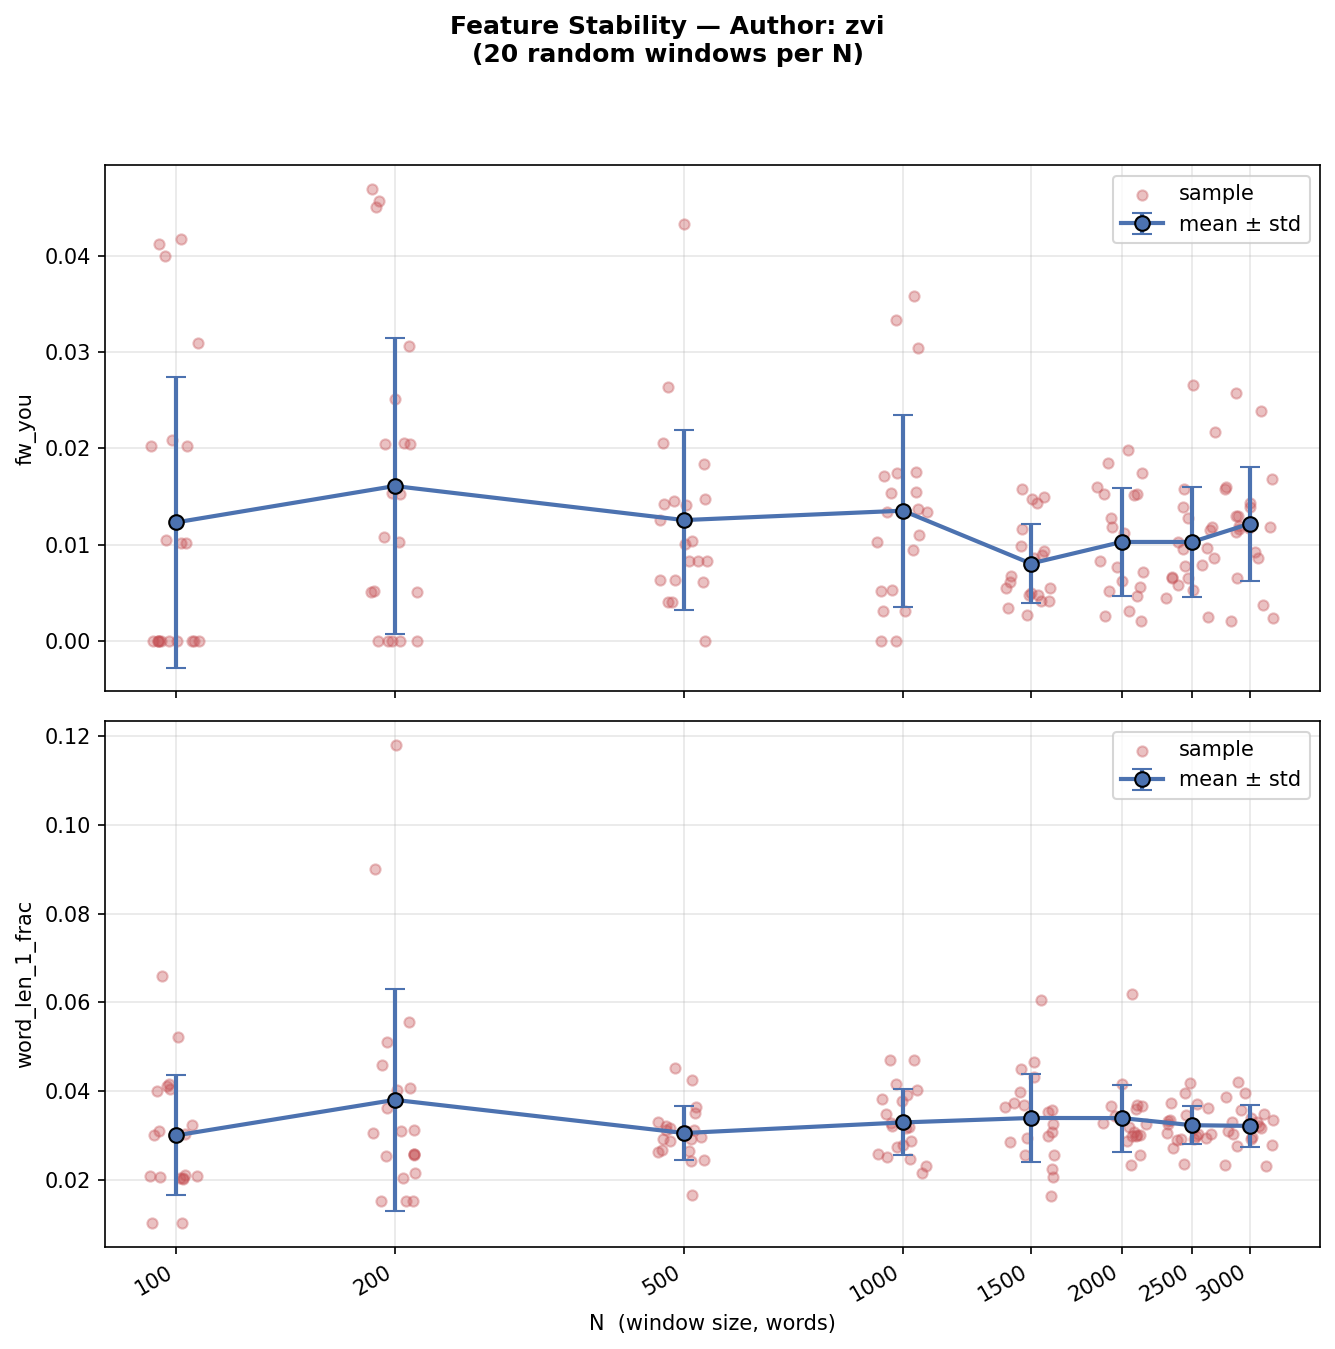
\includegraphics[width=0.75\linewidth]{../outputs/kmeans/effect_of_n/feature_stability_zvi.png}
  \caption{Two stylometric features computed on random windows of \code{zvi}'s
  concatenated text. The spread around each mean narrows as $N$ grows.}
  \label{fig:feat_stability}
\end{figure}

The standard deviation of both features is large at small $N$ and generally shrinks
as $N$ increases. At $N=100$
each window is too short to yield a reliable estimate of \code{zvi}'s rates;
by $N=1500$ the estimates have stabilised.
% =============================================================================
\section{Effect of Era}

Our decision to collect equal numbers of articles from $\leq 2022$ and $\geq 2024$ in the LessWrong 10 Authors dataset stems from a practical observation.
ChatGPT and similar chatbots emerged in late 2022 and quickly gained traction
as writing assistants. By 2024 they were routine tools for many writers, used
to proofread or polish blog posts, emails, and similar texts. Chatbots have a
distinctive style of their own; if a substantial fraction of authors run their
drafts through one, individual writing styles might homogenise. We therefore
hypothesised \textbf{lower K-means performance in the post-2024 era than in
the pre-2022 era}.

\paragraph{Setup.}
LessWrong 10 Authors, $K=4$, $M=10$, $N=1{,}526$, 50 trials per era. Each
trial samples 4 of the 10 authors and 10 of each author's 20 era-restricted
articles; the rest of the pipeline is unchanged. The two eras are sampled
independently, making their error bars statistically comparable.

\begin{figure}[H]
  \centering
  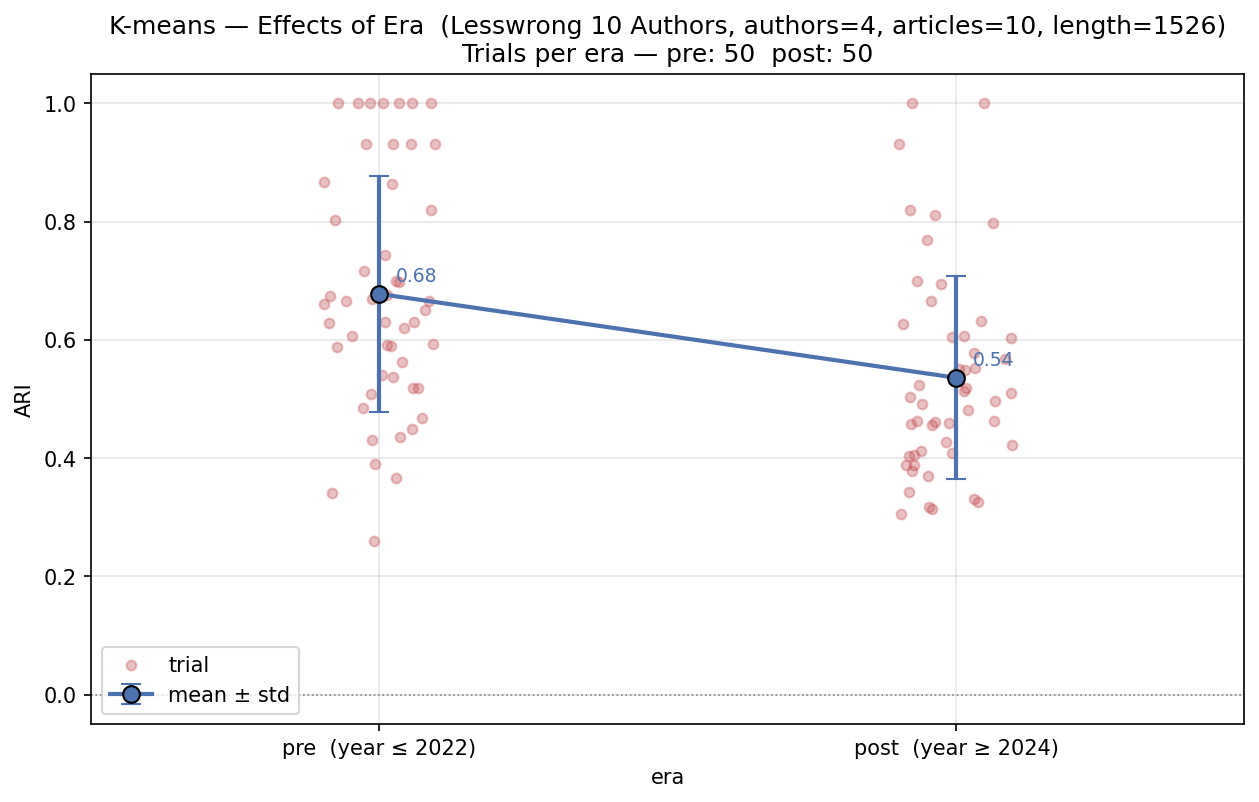
\includegraphics[width=0.82\linewidth]{../outputs/kmeans/effect_of_era/ari_vs_era.png}
  \caption{ARI by era ($K=4$, $M=10$, $N=1526$, 50 trials per era). Mean ARI
  drops from \textbf{0.68} in the pre-2022 era to \textbf{0.54} in the
  post-2024 era.}
  \label{fig:era}
\end{figure}

The mean ARI drops from \textbf{0.68} (pre, $\leq 2022$) to \textbf{0.54}
(post, $\geq 2024$), a substantial gap that is consistent with our expectation.

\paragraph{Does this prove people are using AI to polish their writing?}
Unfortunately, no. The drop is too large to dismiss as noise, but AI use is
only one of several plausible explanations:

\begin{itemize}\setlength\itemsep{2pt}
  \item \textbf{Writing evolves.} Style is not static. An author's prose today
        may not mirror their prose from five years ago simply because they have
        grown intellectually and socially.
  \item \textbf{Topic shifts on LessWrong.} The community's focus has changed
        in response to current events. For instance, \code{kaj\_sotala}'s
        pre-2023 articles are mostly about biology, social dynamics, and
        self-improvement, while his post-2023 articles are mostly about AI.
        A shift in topic mix can drag stylistic features along with it.
\end{itemize}

The era effect is real and worth noting; however, attributing it specifically to
AI-assisted writing would require a controlled study that this experiment
cannot deliver.

\end{document}
